% ===================== PARTE 6: HALLAZGO, COMPARTICIÓN FALSA (diapositivas 63-69) =====================
\parte{Hallazgo: compartición falsa}{Hallazgo: compartición falsa\\en el programa del equipo}
  {Con 10 pilas, \texttt{bench.cpp} rendía 3 veces menos que el programa oficial. La causa era una sola palabra.}{s63}

\begin{frame}{El síntoma: con 10 pilas, \texttt{bench.cpp} rinde unas 3 veces menos}
  \fuente{docker/rendimiento.csv y nativo/rendimiento.csv, 24 hilos; EXPLICACION.md, Parte 6.6}
  \begin{columns}[T]
    \column{0.62\textwidth}\footnotesize\renewcommand{\arraystretch}{1.15}
    \begin{tabular}{@{}lrrr@{}}
      \toprule
      \textbf{24 hilos, Mop/s} & \textbf{Autores} & \textbf{Williams} & \textbf{Libstdc++}\\
      \multicolumn{4}{@{}l}{\scriptsize\color{gris} oficial con Docker $\to$ \texttt{bench.cpp} sin Docker}\\
      \midrule
      $n = 1$ · $u = 1$\,\% & 19,8 $\to$ 21,0 & 4,8 $\to$ 4,0 & 1,2 $\to$ 0,9\\
      $n = 1$ · $u = 10$\,\% & 4,4 $\to$ 5,0 & 1,6 $\to$ 0,9 & 0,6 $\to$ 0,4\\
      $n = 1$ · $u = 50$\,\% & 1,1 $\to$ 1,2 & 0,4 $\to$ 0,2 & 0,2 $\to$ 0,1\\
      \rowcolor{ambarsuave}\textbf{$n = 10$ · $u = 1$\,\%} & \textbf{121,9 $\to$ 35,4} & 34,7 $\to$ 11,4 & 10,8 $\to$ 6,7\\
      \rowcolor{ambarsuave}\textbf{$n = 10$ · $u = 10$\,\%} & \textbf{55,4 $\to$ 18,4} & 16,1 $\to$ 5,8 & 5,4 $\to$ 3,6\\
      $n = \pot{6}$ · $u = 50$\,\% & 55,4 $\to$ 78,8 & 40,4 $\to$ 50,7 & 56,3 $\to$ 82,5\\
      \bottomrule
    \end{tabular}
    \column{0.34\textwidth}
    \caja{Con una pila, Autores coincide. Con 10 pilas rinde \textbf{entre 3 y 3,4 veces menos}. Algo pasa solo cuando hay varias pilas.}
    \par\medskip
    \aviso{Docker no es: el control de la \hyperlink{parte4}{parte 4} dio 1,02\por. El cambio está en el programa.}
  \end{columns}
  \nota{s64}
\end{frame}

\begin{frame}{La causa: 10 pilas comparten 2 líneas de caché}
  \fuente{codigo/bench.cpp, línea 73; tamaños medidos con sizeof; EXPLICACION.md, Parte 6.6}
  \centering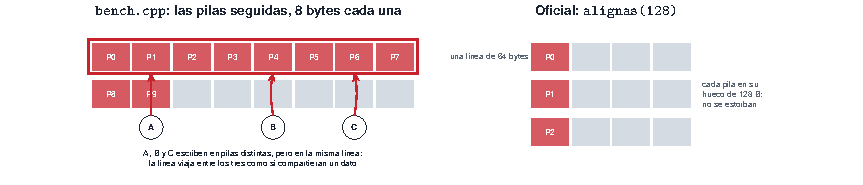
\includegraphics[width=0.9\linewidth]{figuras/s65}
  \par\medskip\raggedright
  \begin{columns}[T]
    \column{0.49\textwidth}\scriptsize\renewcommand{\arraystretch}{1.15}
    \begin{tabular}{@{}lrl@{}}
      \toprule
      \textbf{Algoritmo} & \textbf{Bytes por pila} & \textbf{Las 10 pilas ocupan}\\
      \midrule
      Autores & 8 & 80\,B: \textbf{unas 2 líneas}\\
      Libstdc++, Williams & 16 & 160\,B: unas 3 líneas\\
      Mutex & 56 & 560\,B: unas 9 líneas\\
      \bottomrule
    \end{tabular}
    \column{0.47\textwidth}
    \porque{compartición falsa}{La caché mueve líneas enteras de 64 bytes. Dos datos distintos en la misma línea se estorban aunque nadie los comparta. Con Autores, las «10 pilas» se comportan casi como 2: su diseño compacto juega en su contra.}
  \end{columns}
  \nota{s65}
\end{frame}

\begin{frame}{La prueba: una sola palabra, \texttt{alignas(128)}, en una copia}
  \fuente{nativo y nativo\_alineado/rendimiento.csv (batería completa, 24 hilos); controles.csv (control de alineación)}
  \centering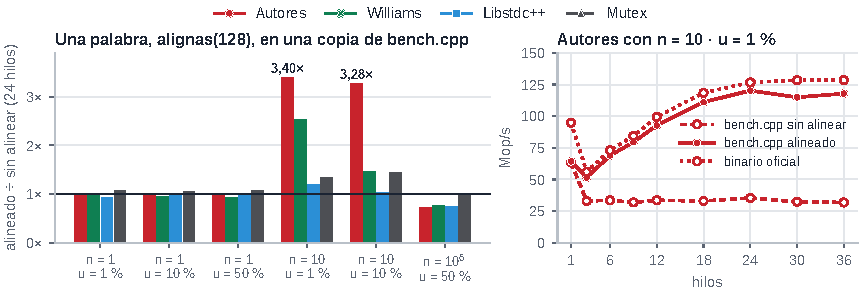
\includegraphics[width=0.9\linewidth]{figuras/s66}
  \vfill\raggedright
  \caja{Con $n = 10$, Autores pasa de 35,4 a \textbf{120,3\,Mop/s (3,40\por)}, casi los 127 del binario oficial. El control: con $n = 1$ no hay pilas vecinas, y la palabra no cambia nada (0,95\por{} a 1,05\por). Si mejorara también ahí, la explicación sería falsa.}
  \nota{s66}
\end{frame}

\begin{frame}{La batería sin alinear: los paneles $n = 10$ miden el programa, no el algoritmo}
  \fuente{nativo/rendimiento.csv; \texttt{bench.cpp} sin Docker, sin alinear, mediana de 5 rondas}
  \centering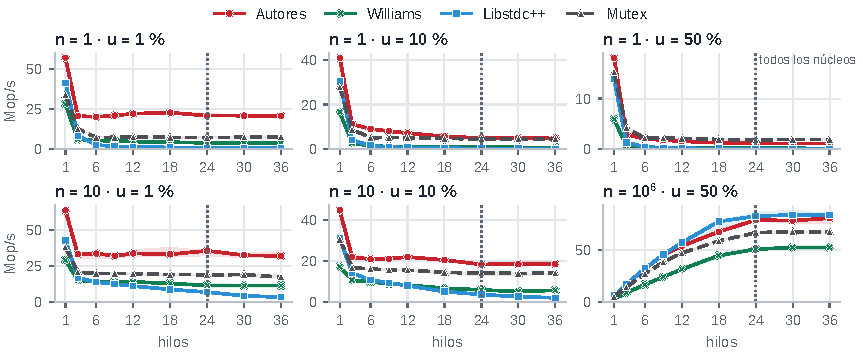
\includegraphics[width=0.9\linewidth]{figuras/s67}
  \nota{s67}
\end{frame}

\begin{frame}{Sorpresa: con un millón de pilas, alinear frena}
  \fuente{nativo\_alineado/memoria\_alineado.csv (herramientas/alinear\_memoria.py); 24 hilos, $u = 50$\,\%, 3 rondas alternadas}
  \centering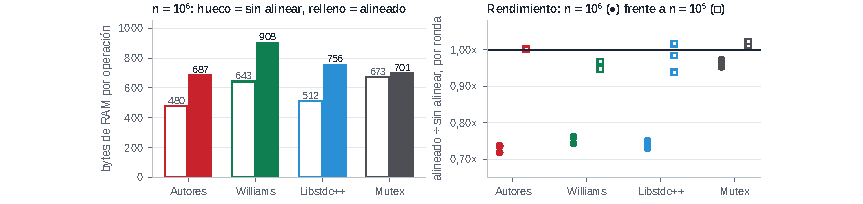
\includegraphics[width=0.9\linewidth]{figuras/s68}
  \par\medskip\raggedright
  \begin{columns}[T]
    \column{0.49\textwidth}
    \porque{ya no cabe en la caché}{Un millón de pilas de 8-16 bytes son 8-16\,MB: caben en los 36\,MB de L3. Con 128 bytes cada una, son 128\,MB: no caben, y muchas operaciones van a la RAM. El Mutex ya ocupaba 56\,MB y no cabía antes: por eso casi no cambia.}
    \column{0.47\textwidth}
    \sub{Dos predicciones, las dos cumplidas}
    \begin{enumerate}\footnotesize
      \item Con \pot{6}, más bytes de RAM por operación: +207 a +265\,B (41-48\,\%), y el rendimiento baja en proporción.
      \item Con \pot{5}, las pilas alineadas ocupan 12,8\,MB y caben: alinear no frena (0,94\por{} a 1,02\por).
    \end{enumerate}
  \end{columns}
  \nota{s68}
\end{frame}

\begin{frame}{Qué cambia este hallazgo}
  \fuente{EXPLICACION.md, Partes 6.6 y 8}
  \begin{columns}[T]
    \column{0.5\textwidth}
    \sub{Para leer los resultados}
    \begin{itemize}\footnotesize
      \item Los paneles $n = 10$ de \texttt{bench.cpp} sin alinear están frenados por el programa: no dicen nada de los algoritmos.
      \item Con \pot{6} pilas, \texttt{bench.cpp} va un 26-46\,\% más rápido que el oficial. Antes se atribuía a sus pilas de 2 nodos; ahora apunta a que sus pilas apretadas caben en la caché. Medido dentro de \texttt{bench.cpp}; frente al oficial sigue siendo una deducción.
      \item Aun con el freno, el orden se mantiene: entre los 3 algoritmos comunes, \texttt{bench.cpp} y el oficial coinciden en quién gana en 49 de 54 puntos.
    \end{itemize}
    \column{0.46\textwidth}
    \sub{Para el equipo}
    \cmd{// codigo/bench.cpp, línea 73\\template <class I> struct alignas(128) Pila}
    \par\smallskip\footnotesize
    Se probó en una copia; \texttt{bench.cpp} no se ha tocado, por la regla del equipo. Queda a su criterio aplicarlo.
    \par\medskip
    \caja{\textbf{Lección general:} en un benchmark concurrente, dónde caen los datos en memoria puede pesar más que el algoritmo.}
  \end{columns}
  \nota{s69}
\end{frame}
